\begin{tikzpicture}[x=0.007cm,y=0.0122cm,
  font=\fontsize{8}{9}\selectfont\sffamily]
\useasboundingbox (-45,70) rectangle (945,920);
\begin{scope}
  \clip (83,130) rectangle (935,906);
  \node[anchor=south west,inner sep=0pt] at (0,0)
    {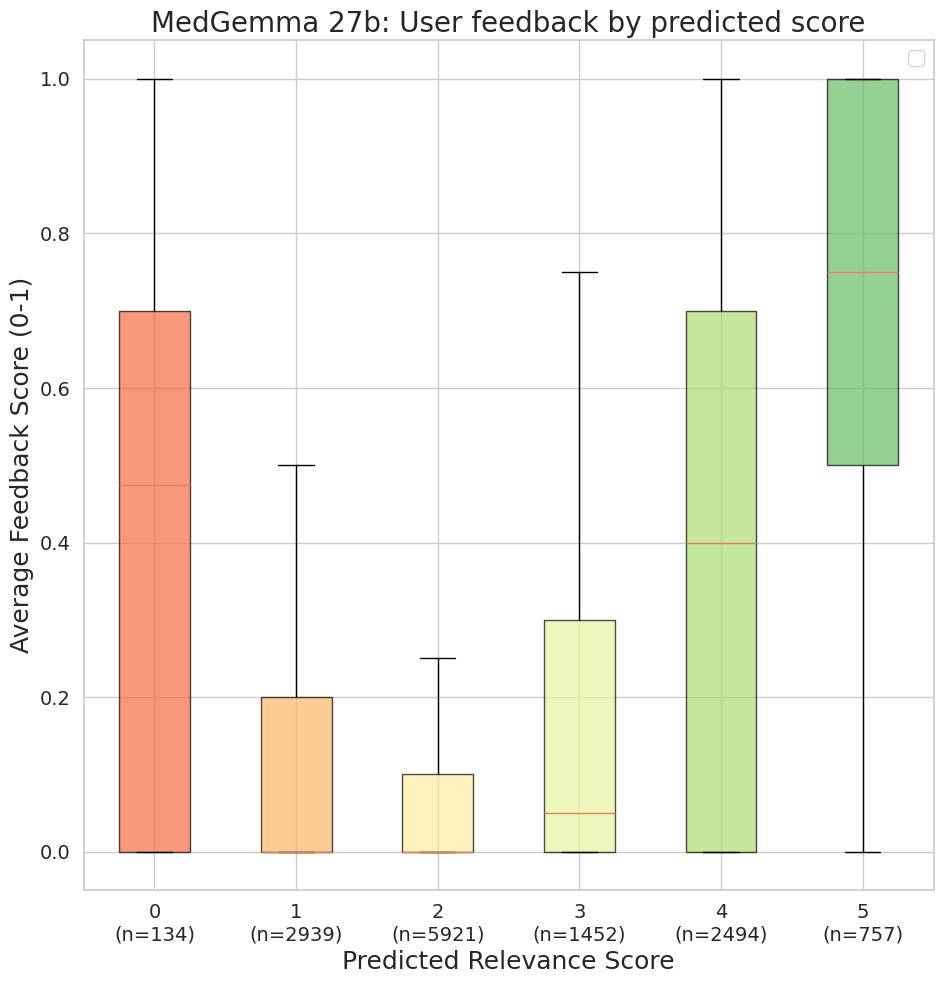
\includegraphics[width=6.601cm,height=12.005cm]{figures/medgemma-vs-feedbackavg.png}};
\end{scope}
\foreach \value in {0,0.2,0.4,0.6,0.8,1} {
  \pgfmathsetmacro{\tickY}{131+774*\value}
  \node[anchor=east,inner sep=2pt] at (83,\tickY) {\value};
}
\foreach \grade in {0,...,5} {
  \pgfmathsetmacro{\tickX}{84+(\grade+0.5)*850/6}
  \node[anchor=north,inner sep=3pt] at (\tickX,130) {\grade};
}
\node[anchor=north,inner sep=0pt] at (509,99) {Teacher grade (MedGemma 27B)};
\node[rotate=90,inner sep=0pt] at (-15,518) {Mean user feedback};
\end{tikzpicture}
